\documentclass[12pt,a4paper]{report}
\usepackage[spanish]{babel}
\usepackage{amsmath}
\usepackage{amsfonts}
\usepackage{amssymb}
\usepackage{makeidx}
\usepackage{cite}
\usepackage{color} 
\usepackage{float}
\usepackage[dvips]{graphicx}
\DeclareGraphicsExtensions{.bmp,.png,.pdf,.jpg}
\usepackage{parskip}
\usepackage[left=2.00cm, right=2.00cm, top=2.00cm, bottom=2.00cm]{geometry}
\author{Valentín Sánchez Ramírez}
\title{Seguridad en vehículos de dos ruedas}
\begin{document}
	
	
	\title{Seguridad en veh\'iculos de dos ruedas}
	\author{
		Valent\'in S\'anchez Ram\'irez\\ \\
		\small{Proyecto Fin de Carrera Ingenier\'ia de Telecomunicaciones}\\ \\
		\small{Dpto. de Electronica y Tecnolog\'ia de Computadores}\\
		\small{Escuela T\'ecnica Superior de Ingenier\'ia Inform\'atica y Telecomunicaicones}\\
		\small{ETSIIT}\\ \\
		\small{Universidad de Granada UGR}\\
	}
	\date{\small{\today}}
	\maketitle
	
	%segunda pagina en blanco y sin numerar
	\newpage
	$\ $
	\thispagestyle{empty} 
	
	\chapter*{}
	\pagenumbering{Roman} %numeracion de paginas en numeros romanos
	
		\textit{Dedicado a	}
	
	%include de indice, resumen, abstract y capítulos
		\tableofcontents % indice de contenidos
	
	\newpage
	$\ $
	

	\cleardoublepage
	\addcontentsline{toc}{chapter}{Índice de figuras} % para que aparezca en el indice de contenidos
	\listoffigures % indice de figuras

	\newpage
	$\ $

	\cleardoublepage
	\addcontentsline{toc}{chapter}{Índice de tablas} % para que aparezca en el indice de contenidos
	\renewcommand{\listtablename}{Índice de tablas}
	\listoftables % indice de tablas
	
	\newpage
	$\ $



	
		\chapter*{Resumen} % si no queremos que añada la palabra "Capitulo"
	\addcontentsline{toc}{chapter}{Resumen} % si queremos que aparezca en el índice
	\markboth{RESUMEN}{RESUMEN} % encabezado
	
	\
	\\
	\
	
	\textbf{Palabras clave:} seguridad en vehículos de dos ruedas, aviso a emergencias, sensor, aplicación móvil, bluetooth, smartphone, unidad inercial.
	
	\
	\\
	\\
	\\
	\
	
	
	Este proyecto fin de carrera propone un sistema de seguridad en vehículos de dos ruedas que permita una rápida intervención de los servicios de emergencias en el caso de sufrir un accidente mientras se circulaba. Hoy en día este aviso se produce si la persona accidentada llama a emergencias o bien si algún testigo llama desde su teléfono personal. El objetivo principal es detectar si se ha sufrido un accidente gracias a la información que suministrará un sistema electrónico situado en el interior de la moto y alimentado por la batería de la misma. La aplicación instalada en el smartphone del usuario será la encargada de recopilar toda la información suministrada por el sistema electrónico, detectar si se ha sufrido un accidente realizando las comprobaciones pertinentes del algoritmo desarrollado y enviar un SMS al número de emergencias indicándoles nuestra ubicación en caso de haber sufrido un accidente.
	

	


	\newpage
	$\ $
	
		\chapter*{Abstract} % si no queremos que añada la palabra "Capitulo"
	\addcontentsline{toc}{chapter}{Abstract} % si queremos que aparezca en el índice
	\markboth{ABSTRACT}{ABSTRACT} % encabezado
	
	
	\
	\\
	\
	
	\textbf{Keywords:} safety two-wheeled vehicles, emergency notification, sensor, mobile application, bluetooth, smartphone, inertial unit.
	
	\
	\\
	\\
	\\
	\
	
	
	
	This end career project proposes a security system in two-wheelers that allows a fast intervention of emergency services in the event of an accident while he was driving.
	
	Today this warning occurs if the casualty emergency call any witnesses or if you call from your home phone.
	
	The main objective is to detect if you have had an accident due to information that will provide an electronic system located inside of the motorcycle and powered by the battery of the same.
	
	The application installed on the smartphone driver will be responsible for gathering all the information provided by the electronics sistem that detect when an accident making the necessary checks of the developed algorithm and send a SMS to the emergency number about our location in case of an accident.
	
	
	
	
	
	\newpage
	$\ $
	
	\chapter{Introducci\'on}\label{cap.introduccion}
	\pagenumbering{arabic} % para empezar la numeración con números
	
		En este cap\'itulo pretendemos situar al lector en el contexto del proyecto, en que campo vamos a trabajar, motivaci\'on y los objetivos del proyecto para que se pueda entender con mayor facilidad el trabajo realizado y los objetivos a conseguir.
		
		Se busca, por tanto, que con la lectura de este cap\'itulo pueda entenderse el resto de esta memoria.
		
	\section{Motivaci\'on}
		
		Desde la invenci\'on de la motocicleta por Sylvester Howard Roper en 1867, el mundo del motor ha evolucionado desde el motor de cilindros a vapor hasta los motores actuales. Diferentes tipos de motocicletas con distintas cilindradas inundan nuestras calles a d\'ia de hoy.
		
		Como podemos ver al salir a la calle las motocicletas no son el \'unico veh\'iculo que nos encontramos, tambi\'en podemos encontrar coches, camiones y sus variantes en forma, motor, tama\~no y n\'umero de ruedas. Lo que si podemos observar es que la moticleta es el veh\'iculo menos seguro frente a los mencionados, no solo por dimensiones sino porque en caso de accidente es el cuerpo del motorista quien sufre el impacto y no la carrocer\'ia como en los otros veh\'iculos.
		
		Con el paso de los a\~nos la seguridad en veh\'iculos con motor ha aumentado progresivamente. Este crecimiento ha sido mayor con la introducci\'on de nuevas tecnolog\'ias, tales como sensores, dotan al veh\'iculo de cierta inteligencia.
		
		A la hora de usar un veh\'iculo de dos ruedas lo mas importante es nuestra seguridad, prueba de ello son los sistemas que se est\'an implantando tanto en el propio veh\'iculo como en cascos o chaquetas. En el caso de sufrir un accidente el tiempo juega en nuestra contra, una r\'apida actuación de los servicios sanitarios puede salvarnos la vida en caso de que lo necesitemos.
		
		Al a\~no se producen mas de 2000 accidentes de moto, el 72\% de esos accidentes precisa atenci\'on m\'edica. Algunos veh\'iculos de alta gama ya poseen un sistema de seguridad en caso de sufrir en accidente, sistema que ser\'a obligatorio en Espa\~na a partir del 31 de Marzo de 2018 en coches. Quedando disponible realizar un sistema parecido para motos, el cual podr\'ia llegar a ser obligatorio en un futuro.
		
		Hoy en d\'ia es dif\'icil encontrar una persona que no posea un smartphone, una herramienta que no solo sirve para llamar, leer la prensa o encontrar una ubicaci\'on, sino que con la posibilidad del desarrollo de aplicaciones podemos convertir nuestro smartphone en una herramienta que nos ayude en cualquier tarea, circunstancia o incluso que nos salve la vida.
		
		Si combinamos la tecnolog\'ia de nuestro smartphone con un sistema electr\'onico que pueda ser integrado en una moto, ya sea desde el momento de su fabricaci\'on o un extra, aumentariamos la seguridad de todo motorista.
		
		Es cierto que no disminuiriamos el números de accidentes que puedan ocurrir en carretera, pero si disminuir\'iamos el tiempo de reacci\'on de los servicios sanitarios, aumentando las probabilidades de atender a una persona en el menor tiempo posible.
		
	\section{Descripci\'on del proyecto}
	
		Como se ha indicado, es muy importante el tiempo de reacci\'on de los servicios de emergencias, facilitando ademas nuestra ubicaci\'on ayudamos a que nos encuentren con facilidad en caso de estar en alg\'un lugar de dif\'icil acceso, que no hayamos podidos llamar por nuestros medios o que no hubiera testigos de dicho accidente que pudieran llamar a emergencias para informar de la gravedad de lo ocurrido.
		
		Adem\'as debemos tener en cuenta que este sistema funciona solo, no necesita de la intervenci\'on del motorista una vez el sistema ha sido iniciado en caso de accidente.
		
		Para que este sistema sea efectivo es preciso que el motorista circule con un smartphone encendido, conectado v\'ia bluetooth al sistema electr\'onico integrado en la motocicleta y con la aplicaci\'on iniciada.
		
		Este proyecto pretende ser un sistema completo y aut\'onomo que se componga de un sistema electr\'onico, compuesto por un gir\'oscopo, magnet\'ometro y aceler\'ometro, capaz de transmitir v\'ia bluetooth a un smartphone todos los par\'ametros necesarios para que la aplicaci\'on desarrollada ejecute el algoritmo implementado.
				
		Por ello podemos decir que los elementos clave para aumentar la seguridad en un veh\'iculo de dos ruedas y reducir el tiempo de intervenci\'on de los servios de emergencias en este proyecto ser\'ian:

		\begin{itemize}
			\item Sensores.
			\item Bluetooth.
			\item Smartphone.
		\end{itemize}
		
		Adem\'as, es necesario que el smartphone posea GPS, para una vez los datos han sido recibidos y almacenados, podamos operar con ellos en nuestro algoritmo, el cual nos comprobar\'a si hemos sufrido un accidente en base a nuestro \'angulo de inclinaci\'on y la velocidad a la que circulamos. En caso que el algoritmo detecte haber sufrido un accidente enviar\'a un SMS a los servicios de emergencias indic\'andoles la ubicaci\'on recogida por el GPS.
	
	
	\section{Objetivos}
	
		En este proyecto, se pretende entrar en contacto con el dise\~no y programaci\'on de una placa Arduino UNO, la interpretaci\'on de los datos que proporciona el Pololu MinIMU-9 v2, establecer la comunicaci\'on Bluetooth entre la placa Arduino UNO y un dispositivo Android y la programaci\'on y dise\~no de la app m\'ovil en Android.
	
		Para ello conectaremos el Pololu MinIMU-9 v2 y el dispositivo Bluetooth HC-05 a la placa Arduino UNO, programaremos nuestra placa Arduino para que reciba los datos del sensor y los env\'ie mediante Bluetooth al dispositivo Android.
		
		Posteriormente debemos programar una app Android en nuestro Smartphone que sea capaz de conectarse al dispositivo HC-05 y leer la informaci\'on recibida, esta app ser\'a la encargada de ejecutar el algoritmo y comprobaciones pertinentes. En caso de haber sufrido un accidente se le notificara al n\'umero de emergencias 112 de nuestra ubicaci\'on via SMS.
		
		Para llevar a cabo este proyecto, el trabajo a realizar se divide en los siguientes objetivos:
		
		\begin{itemize}
			\item Instalaci\'on de entorno Arduino y familiarizarse con dicha programaci\'on. Estudio de la programaci\'on Arduino para leer los datos recibidos de la mota sensora y enviarlos via Bluetooth.
			
			\item Estudio de las bibliograf\'ia acerca de la calibrac\'on de los sensores y de los algoritmos de c\'alculo de Pitch, Roll y Yaw. Se estudiar\'a el funcionamiento de las motas y como deben ser programadas.
			
			\item Montaje de la mota sensora y HC-05. Montar la mota sensora y el m\'odulo HC-05 y tenerlos listos para su uso, realizaci\'on de programas b\'asicos de prueba y verificaci\'on de que funcionan correctamente. Se dispondr\'a de una protoboax para las pruebas pertinentes hasta el desarrollo de una placa en PCB para posterior implementaci\'on.
			
			\item Estudio de programaci\'on Android en Eclipse. Con la correspondiente app que ejecute nuestro algoritmo de detecci\'on de accidente y en caso necesario enviar la ubicaci\'on actual a Emergencias 112 via SMS.
			
			\item Pruebas del sistema en diferentes condiciones. Realizaci\'on de las pertinentes pruebas para comprobar el correcto funcionamiento del sistema desarrollado. Pruebas a diferentes velocidades, diferentes \'angulos de inclicaci\'on del sistema electr\'onico que ir\'a integrado en la moto. Adem\'as de pruebas del sistema en diferentes circunstancias meteorol\'ogicas para comprobar el alcande del dispositivo bluetooth.
			
			\item Desarrollo de PCB's. Desarrollo de una placa PCB para evitar el uso de cables en el proyecto y hacerlo mas compacto.
			
		\end{itemize}
		
		Adem\'as los objetivos que debemos cumplir de cara a la comercializaci\'on de este proyecto ser\'ian los siguientes:
		
		\begin{itemize}
			\item Acabado sistema electr\'onico: debe ser un sistema de tamaño reducido, de facil ingraci\'on a una moto y con una entrada de alimentaci\'on desde la bater\'ia.
			
			\item Comodidad de uso de cara al usuario: el individuo que disponga de dicho proyecto, solo debe preocuparse de emparejar el bluetooth de su smartphone con el bluetooth del sistema electr\'onico, despues de ello, solo debe encender la aplicaci\'on antes de circular con su moto y apagarla una vez haya llegado a su destino. 
			
			\item Monitorizaci\'on en tiempo real: se requiere de una comunicaci\'on en tiempo real entre smartphone y sistema electr\'onico, para que se pueda actuar en la mayor brevedad posible.
			
			\item Movilidad: la aplicaci\'on puede ser instalada en cualquier dispositivo portatil Android que posea bluetooth, GPS y pueda enviar SMS, por lo que debe poseer una tarjeta SIM que posibilite el uso de la red telef\'onica.
			
			\item Disponibilidad, robustez y eficiencia: el sistema debe ser tolerante y recuperable a fallos. Por un ejemplo un fallo puede ser la p\'erdida de comunicaci\'on bluetooth momentanea, por lo que se reconoce como un fallo puntual y no como un accidente. La transmisi\'on de datos debe diseñarse con una estructura lo mas eficiente posible, con una buena sincronizaci\'on. Adem\'as se debe desarrollar una interfaz de la aplicaci\'on intuitiva.
			
			\item Interpretabilidad de los datos: no solo la monitorizaci\'on en tiempo real es necesaria para el correcto funcionamiento del algoritmo implementado. Una buena y r\'apida interpretabilidad de los datos es fundamental. En esta versi\'on de prueba los datos se mostrar\'an en diferentes TextView, posibilitando as\'i la interpretaci\'on de los datos y poder ver el comportamiento del algoritmo en funci\'on de los datos recibidos.
			
		\end{itemize}
		
	\newpage
	$\ $
	
		\chapter{Estado del arte}\label{cap.estadoDelArte}
	
	En este capítulo vamos a realizar un estudio de la situación tecnolólogica actual en todo lo referente a la comunicación inalámbrica existente y los sistemas de seguridad actuales. Además veremos los distintos sistemas que trabajan con unidades inerciales para el cálculo de ángulos, a parte de una comparación entre giróscopos manuales y digitales.
	
	\section{¿Qué es una IMU?}
	
		Una Unidad de Medidas Inerciales (IMU o UMI en español) es en general un sistema cerrado que es usado para detectar la orientación, localización y movimiento. Este dispositivo normalemente usa una combinación de acelerómetros y sensores de velocidad angular (giroscopos) para conocer como se está moviendo éste y en que posición se encuentra.
		
		Una IMU detecta la aceleración y los cambios de orientación instantáneamente (ángulos roll, pitch and yaw), además los intregra para averiguar el cambio total sobre la posición inicial. Esto contrasta con el sistema GPS, el cual utiliza los satélites para detectar la posición.
		
		Las IMUs por tanto suelen tener un error acumulado o deriva. Porque una IMU esta sumando continuamente los cambios detectados en la posición, cualquier error en esta medida es acumulado. Esto da lugar a la “deriva”, o un error creciente entre la posición hallada por la IMU y la posición real de ésta.
		
		Las IMUs son normalmente un componente de un sistema de navegación. Otros sistemas tales como los GPS (usados para corregir el término de deriva en la posición), un sistema barométrico (para la corrección de la altitud), o un compás magnético (para la corrección de la orientación) compensan las limitaciones de una IMU. Hay que notar que la mayoría de los otros sistemas tienen sus propios defectos los cuales son compensados entre ellos.
		
		El término IMU esta ampliamente extendido para referirse a una caja, la cual contiene 3 acelerómetros. Estos están situados de tal forma que sus ejes de medida son mutuamente ortogonales. Miden las llamadas “fuerzas específicas” (aceleración inercial – gravedad). 
		
		Tres giróscopos están situados de forma que sus ejes de medidas sean ortogonales entre sí midiendo las velocidades de rotación.
		
		La integración de la estimación de la velocidad angular en los giróscopos causará el error de deriva, pero la observación del vector gravedad mediante acelerómetros sirve como una observación externa de la vertical en un punto (local). Esto corrige la mayoría de los errores de deriva. Se incluyen también uno o más sensores de temperatura, pueden estar incorporados en cada acelerómetro o giróscopos, o como un sensor adicional usado para calibrar los datos de lectura/escritura de los otros sensores.
		
		Para conseguir una precisión superior, la caja debe ser diseñada de forma que la temperatura sea controlada y se mantenga constante. Las paredes de la caja están hechas de materiales que minimicen la interferencia electromagnética. Si las señales de salida son analógicas, el ruido eléctrico debe ser minimizado en los cables y en el conversor analógico-digital. Si la señal de salida esta ya en formato digital, el retraso temporal se convierte en la principal preocupación.
		
		Los datos suministrados por una caja de IMU es todo lo que se necesita para llevar a cabo la estimación de la navegación. El primer uso de tal caja fue en un barco, y todavía casi todos los barcos tienen una. Los satélites también tienen una. Casi cualquier cosa que debe usar de alguna manera la electrónica para saber su aceleración, orientación y/o velocidad tiene una IMU. 
		
		Dada la variedad de situaciones en las que se hace necesaria una IMU, y las peculiaridades que presentan cada una de ellas, el concepto de IMU no está claramente definido. Suele estar englobado en un sistema de navegación inercial, pero su papel en éste puede variar sustancialmente. La caja de sensores de aceleración y velocidad angular ya constituye una IMU. Si modificamos las ecuaciones cinemáticas y aplicando los datos a un filtro de Kalman, dichos datos de la IMU pueden ser transformados para obtener el roll, el pitch y el yaw. A esto también se le llama sistema ARS (Sistema de referencia para orientación). En ambientes dinámicos tales como un jet de combate, la gravedad será enmascarada por la aceleración del cuerpo del avión. En estos casos la IMU está normalmente acoplada con un GPS u otros sensores. Esto nos conduce un poco más cerca de los sistemas de navegación y de dirección y nos aleja de las IMU. Este es el motivo de por qué la mayoría de los ingenieros no hacen diferencia entre una IMU y un sistema de dirección inercial.
		
		En nuestro caso, la IMU se encargará de proveer al sistema de una referencia de orientación, y será la propia aplicación del smartphone la encargada de estimar el ángulo de inclinación y la velocidad de circulación, en función de los datos del GPS. 



	\section{Sistemas actuales que trabajan con IMUs}	
	
		\subsection{Plataforma giroestabilizada en tres ejes}
	
		Algunos sistemas sitúan los acelerómetros en una plataforma giroestabilizada. Los giroestabilizadores son un conjunto de tres anillos, cada uno de los cuales lleva un par de cojinetes. Estos permiten a la plataforma rotar sobre cualquier eje en el espacio. Normalmente hay dos giroscopios en la plataforma.

		Estos dos giroscopios se usan para cancelar la precesión giroscópica, la tendencia de un giroscopio a girar perpendicularmente a una fuerza sufrida. Montando un par de giroscopios (con la misma inercia rotacional y giro, a la misma velocidad) en ángulo recto las precesiones se cancelan, y la plataforma se mantendrá.
		
		Este sistema permite que los ángulos de roll, pitch y yaw de un vehículo sean medidos directamente. Se pueden usar circuitos electrónicos relativamente simples para obtener las aceleraciones lineales, esto es porque las direcciones de medida de los acelerómetros lineales no cambian.
		
		El inconveniente de este tipo de sistema es que usa muchas partes mecánicas de precisión que son muy caras. Además tiene partes móviles que se pueden estropear, y es vulnerable a que un giroestabilizador se bloquee. El sistema de guiado primario del cohete Apollo usaba una plataforma giro estabilizada de tres ejes, la cual suministraban datos al ordenador de guiado del Apollo.
		

	
	\section{Investigaciones actuales con IMUs}
	
		\subsection{Unidad de medida inercial inalámbrica para cohetes} 
		
		Normalmente tomar el rango de un cohete es un proceso costoso, ya que no proporcionan unas medidas precisas de su posición, velocidad y altitud. De ahí que se usen actualmente sistemas radar en tierra que si proporcionan una información mas precisa en el lo referente al tiempo, posición y velocidad, mientras que para calcular la altitud se basan en las imagenes tomadas en un video a camara lenta, por lo que resulta dificil calcular con precisión su altura. 
		
		La miniaturización lograda por las nuevas técnicas de fabricación hace que sean dispositivos atractivos para ser implementados en un sistema de seguimiento y medición de las dinámicas del movimiento de un pequeño cohete, estos sistemas se conocen como Strapdown, término que se refiere a que el sistema de medida se encuentra ajustado al marco de referencia del objeto en prueba, es decir, se mueve de la misma forma que lo hace dicho objeto.
		
		Como ejemplo de ello, se tiene el Intersense, que es un sistema de seguimiento inercial-acústico, que aprovecha las nuevas características de los sensores inerciales y que logra su difusión comercial en aplicaciones de seguimiento. El IMU desarrollado está basado en el concepto Strapdown. \cite{Cohete}
		
		
		\subsection{Desarrollo de un sistema de giroscopios digitales usando tecnología fpga para monitoreo de la orientación de robots}

		El objetivo de este trabajo es la descripción en VHDL e implementación en FPGA de una unidad de pre-procesamiento digital capaz de disminuir el error en las mediciones realizadas por un giroscopio digital de tres ejes tipo MEMS aumentando la exactitud de éstas para posteriormente obtener la orientación del sensor que al ser montado en un robot se obtendrá la orientación de éste. 
		
		Se emplearon métodos estadísticos para calcular y eliminar el nivel de offset en cada una de los ejes del giroscopio, así como las técnicas de Diezmado, filtro Butterwoth y filtro Kalman para eliminar el ruido eléctrico en las señales., Para la validación del sistema el giroscopio se montó en la flecha de un motor de CD con encoder con el que se realizaron pruebas de velocidad y se compararon los resultados donde se obtuvo como resultado una considerable reducción en la variación de alta frecuencia (ruido) en las medidas del giroscopio así como un nivel de referencia de cero en la señal gracias a la eliminación del offset. Con esta unidad de procesamiento se obtiene un acondicionamiento de la señal listo para ser utilizadas por algún sistema digital que requiera la aplicación del giroscopio, en el caso de este trabajo las señales son integradas por in sistema digital para obtener la orientación de un robot manipulador en los ejes Roll, Pitch y Yaw en un marco de referencia. \cite{robots}		
	
	

	
	\section{Sistemas de seguridad actuales y tendencias futuras}
	
		La tecnología comienza a subirse a la moto, la comunicación entre vehículos y carreteras contribuirá a la prevención de accidentes y disminución de la siniestralidad de uno de los colectivos más vulnerables.
		
		La implantación de sistemas de seguridad como el cinturón de seguridad, airbag, ABS, entre otros muchos han sido incorporados de forma tardía en la moto. La década en la que nos encontramos se centrará en la moto, los sistemas inteligentes van a tener un papel especial.
		
		En materia de seguridad activa, la que ayuda a evitar accidentes hay que destacar los sistemas de ayuda en la frenada, además de la implantación de mejoras en materia de iluminación, amortiguación, estabilidad, sistemas de cambios, neumáticos... En prueba se encuentran algunos sistemas novedosos basados en la comunicación entre vehículos y con las infraestructuras para advertir sobre situaciones peligrosas como tráfico, climatología adversa...
		
		En los últimos dos años se ha iniciado una revolución electrónica en la motocicleta, aportando una gran seguridad como es el ABS, control de tracción. En 2017 la UE (Union Europea) trabaja para que las motos salgan con el ABS de fábrica.
		
		En materia de seguridad pasiva nos encontramos elementos como el casco, la cabeza sufre traumatismos en el 50\% de los accidentes. Un casco adecuado puede reducir estas lesiones en un 69\% y la mortalidad en un 42\%. Ademas de ropa ligera que protege en las caidas o incluso cazadoras, chalecos y cascos con airbag en caso de caida.
		
		\begin{figure}[h]
			\centering
			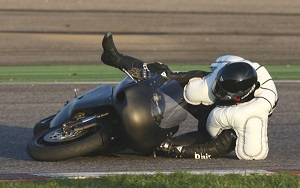
\includegraphics{imagenes/airbag.jpg}
			\caption{Airbag en casco y cazadora}
			\label{contexto:figura}
		\end{figure}
		
		Toda esta información ha sido recopilada de un reportaje de la DGT \cite{Dgt}.
		
		Tal y como hemos podido leer todos estos sistemas en materia de seguridad activa y pasiva son para preveer accidentes o reducir los da\~nos sufridos en caso de accidente. Si el motorista ha sufrido un accidente el tiempo juega en su contra, por lo que se requiere una rápida intervención de los servicios sanitarios. 
		
		Un accidente puede ocurrir en un lugar concurrido y cualquier viandante que se encuentre allí puede realizar dicha llamada a emergencias, el inconveniente sería que el accidente ocurra en una via poco transitada y el conductor no pueda realizar dicha llamada, esperar a que otro conductor circule por esa misma via puede llevar demasiado tiempo.
		
		Como consecuencia nace la realización de este proyecto, cuya aplicación he llamado MotoSafe. Consiste en que el propio smartphone del conductor pueda avisar a emergencias indicándoles nuestra posición en caso que la aplicación haya detectado que se ha producido un accidente a partir de los datos suministrados por el sistema electrónico que ubicaremos en la moto.
		
		En el próximo capítulo se proporcionarán mas detalles acerca del desarrollo de este proyecto.
		
		A continuación detallaré algunos sistemas actuales de alerta móvil en caso de accidentes de tráfico.
		
		\subsection{My-AlarmMe!}
		
			MyAlarmMe! \cite{MyAlamMe} es un sistema de alarma y emergencia para moteros que funciona a través del teléfono móvil.
			
			\begin{figure}[h]
				\centering
				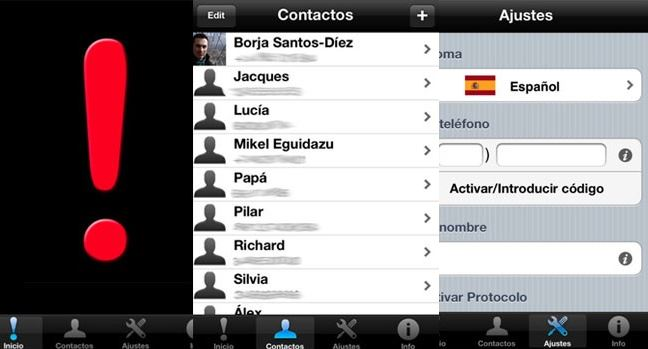
\includegraphics{imagenes/alarm.JPG}
				\caption{Interfaz de My-AlarmMe}
				\label{contexto:figura}
			\end{figure}
			
			Ofrece un servicio personalizado que permite al usuario avisar, en tiempo real y de forma manual, a todas que personas que el desee con el envío de un SMS que ha sufrido un accidente.
			
			Los sms se enviarán de forma automática al acticar tu alarma, el mensaje enviado será prefijado por el usuario incluyendo el nombre de dicho usuario y las coordenadas de su ubicación.
			
			El funcionamiento es simple, una vez la aplicación ha sido configurada, en caso de sufrir un accidente el usuario solo tiene que abrir la aplicación y pulsar sobre el icono de exclamación, en ese momento se enviarán los sms a los contactos o números previamente indicados.
			
			
		
		\subsection{MEC –- Mobile Emergency Call}
		
			MEC -- Mobile Emergency Call \cite{MEC} es una aplicación que envía mensaje de alarma automaticamente si detecta que hemos tenido un accidente de tráfico. Los mensajes de alerta que envía son por medio de email, SMS y llamada de voz con locución incorporada.
			
			Este sistema se puede usar en coches, motos y bicicletas, teniendo en cuenta las particularidades dinámicas y de conducción de cada vehículo. Si el algoritmo detecta un accidente se inicia una cuenta atrás para enviar los mensajes de alerta, cuenta atrás que puede ser cancelada si el usuario así lo indica.
			
			En esos mensajes de alerta se incluyen la posición GPS del accidente, además de los datos de usuario previamente insertados, como son el modelo de vehículo, alergias conocidas, etcétera. El usuario puede escoger a quien desea enviar dichos mensajes de alerta.
			
			\begin{figure}[h]
				\centering
				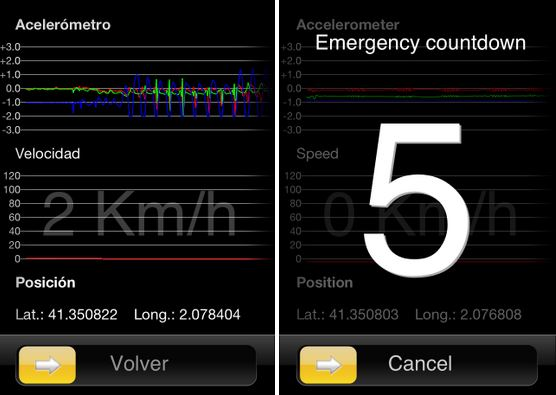
\includegraphics{imagenes/mec.JPG}
				\caption{Interfaz MEC - Mobile Emergency Call}
				\label{contexto:figura}
			\end{figure}
			
		
		
		\subsection{Bosch Media Service}
		
			Bosch \cite{Bosch} ofrece la primera unidad de medición inercial para motocicletas fabricadas en serie. Este sensor proporciona la información necesaria para ofrecer un nivel significativamente mayor de seguridad y comodidad, así como un mayor rendimiento.
			
			Para proporcionar esta información, la unidad de medición inercial MM5.10 mide las señales inerciales 5D, la velocidad de balanceo, la velocidad de viraje, la aceleración longitudinal, la aceleración transversal y la aceleración vertical de la motocicleta. El ángulo de inclinación y el ángulo de cabeceo también se pueden calcular mediante un microcontrolador. La información sobre las velocidades de las ruedas y otros parámetros específicos de la motocicleta (tamaño y forma de los neumáticos y la ubicación de la instalación geométrica del sensor) son necesarios para este cálculo. Todas las señales se transmiten a través de CAN.
			
			Gracias a esta información, es posible obtener y mejorar un gran conjunto de funciones:
				
				\begin{itemize}
					\item Control de tracción
					\item ABS en curvas
					\item Ajuste de wheelie
					\item Ajuste de puesta en marcha
					\item Distribución de la fuerza de frenado en inclinación
					\item Luces de giro
					\item Ajuste del chasis semiactivo
					\item Control en pendientes
					\item Detección de caídas
			    \end{itemize}

	\newpage
	$\ $
	
		\chapter{Desarrollo del Proyecto}\label{cap.desarrollo}
	
	Érase una vez...
	\section{sección1}
	Bla bla bla
	\subsection{subsección1}
	Ble ble ble
	\subsubsection{subsubsección1}
	Bli bli bli
	\paragraph{párrafo1}
	Blo blo blo



	\newpage
	$\ $
	
		\chapter{Resultados}\label{cap.resultados}
	
	En este cap\'itulo vamos a analizar los datos obtenidos de este proyecto, adem\'as de proporcionar una comparaci\'on entre los datos te\'oricos ofrecidos por el fabricante y los datos obtenidos tras su implementaci\'on con la realizaci\'on de pruebas de evaluaci\'on y an\'alisis de dichos resultados.
	

	
	\section{Resultados Hardware}
	
	Dentro de Hardaware debemos distinguir los dos componentes mas importantes que poseemos como son el dispositivo bluetooth HC-05 y la mota sensora.
	
	En lo que respecta al dispositivo bluetooth HC-05 \cite{HC05} como pude estudiar su alcance era de 10 metros, pero en un entorno abierto he podido comprobar que su alcance se reduce a unos 8 metros aproximadamente, a pesar de evitar el apantallamiento con el plano masa dise\~nado en la PCB.
	

	
	\begin{figure}[h]
		\centering
		\includegraphics[5cm,0cm][7cm,9.5cm]{imagenes/theta0.jpg}
		\caption{Theta te\'orico 0}
		\label{contexto:figura}
	\end{figure}
	
	Comprobamos el funcionamiento de la mota sensora, para ellos partimos de dos angulos iniciales y comprobamos la tendencia de las medidas del sensor transcurridos 30 minutos y sin variar la posici\'on del dispositivo.
	
	\begin{figure}[h]
		\centering
		\includegraphics[5cm,0cm][7cm,10cm]{imagenes/theta90.jpg}
		\caption{Theta te\'orico 90}
		\label{contexto:figura}
	\end{figure}
	
	Tal y como podemos observar en las fuguras 4.1 y 4.2 transcurridos 30 minutos el sensor tiende a variar 0.1 grados con respecto al \'angulo inicial de partida. He de destacar que los \'angulos te\'oricos y pr\'acticos difieren debido al desnivel involuntario que pos\'ee la mesa donde realic\'e las pruebas.
	
	
	
	\section{Resultados Aplicaci\'on Android}
	
		En lo que respecta a los resultados de la aplicaci\'on Android vamos a detallar algunas de las situaciones ya explicadas en el cap\'itulo desarrollo sobre como se comporta nuestra aplicaci\'on en diferentes circunstancias, mostrando una captura de pantalla de la interfaz en ese instante.
		
		Veremos los siguientes casos:
		
		- Si el GPS est\'a desactivado.
		
		- Si no se detecta accidente.
		
		- Posibilidad de accidente por p\'erdida de señal.
		
		- En caso de sufrir un accidente, como se comporta la aplicaci\'on.	
		
		\subsection{GPS desactivado}
		
			En el caso de encontrar el sistema GPS de nuestro smartphone desactivado, nos aparecer\'a un alert, ofreciendonos la posibilidad de activarlo en ese instante. Ver figura 4.3.
		
			\begin{figure}[h]
				\centering
				\includegraphics[5cm,0cm][7cm,18cm]{imagenes/GPSOff.png}
				\caption{Interfaz aplicaci\'on Android si el GPS no est\'a activado}
				\label{contexto:figura}
			\end{figure}
			
			Si pulsamos sobre ''No'' la aplicaci\'on se cerrar\'a autom\'aticamente, en caso de pulsar sobre '' Menu de opciones GPS'' accdemos a la secci\'on de ajustes del smartphone para poder encenderlo y continuar usando la aplicaci\'on.
			
			Hemos de tener en cuenta que si no activamos el GPS, ya sea desde esta opci\'on o previamente no podremos usar la aplicaci\'on MotoSafe.
		
		\subsection{No se detecta accidente}
		
			Una vez nuestra aplicaci\'on comienza a funcionar, mide el \'angulo de inclinaci\'on de la motocicleta. Ver figura 4.4.
		
			\begin{figure}[h]
				\centering
				\includegraphics[5cm,0cm][7cm,18cm]{imagenes/NoAccidente.png}
				\caption{Interfaz aplicaci\'on Android reconociendo \'angulo de inclinaci\'on}
				\label{contexto:figura}
			\end{figure}
			
			Tal y como se puede observar en la figura 4.4, en el primer TextView, el \'angulo de inclinaci\'on medido es 0,1217 grados, lo cual indica que permanecemos sobre la vertical y nuestra inclinaci\'on es pr\'acticamente nula.
			
			Adem\'as el segundo TextView reconoce que no se ha sufrido una caida y nos muestra dicho mensaje para poder ver el funcionamiento de la aplicaci\'on.
		
		\subsection{Posibilidad de accidente por p\'erdida de se\~nal}
		
			Muchos son los motivos por los que se puede perder la comunicaci\'on entre el smartphone y el dispositivo que integraremos en la moto, lo cual debemos tener en cuenta para evitar el env\'io de falsos mensajes de accidente al n\'umero de emergencias. Ver figura 4.5.
		
			\begin{figure}[h]
			\centering
			\includegraphics[5cm,0cm][7cm,15cm]{imagenes/perdidaBT.png}
			\caption{Interfaz aplicaci\'on Android con p\'erdida de se\~nal bluetooth}
			\label{contexto:figura}
			\end{figure}
			
			Como se puede apreciar en \'esta figura, la aplicaci\'on reconoce la p\'erdida de comunicaci\'on, mostrando el mensaje ''perdida de BT'', adem\'as seg\'un el algoritmo que he implementado reconoce como que a\'un no se ha caido como se puede apreciar en el segundo TextView, pero tal y como se pudo ver en el diagrama de estados del cap\'itulo desarrollo, el algoritmo pasa a comprobar la velocidad a la que circulamos, muestra de ello es el mensaje ''mido velocidad'' que se encuentra en el tercer TextView.
		
		\subsection{Accidente y aviso a emergencias}
		
			Una vez hemos detectado dicho que ha ocurrido un accidente, ya sea por la p\'erdida de comunicaci\'on o un \'angulo de inclinaci\'on superior a 55 grados y una velocidad menor a 3 metros por segundo, podemos ver la siguiente interfaz. Ver figura 4.6.
		
			\begin{figure}[h]
				\centering
				\includegraphics[5cm,0cm][7cm,15cm]{imagenes/accidente.png}
				\caption{Interfaz aplicaci\'on Android cuando he sufrido un accidente}
				\label{contexto:figura}
			\end{figure}
			
			En el cuarto TextView se muestra el SMS que ha sido enviado al n\'umero de emergencias.
	
	\section{Prototipo}
	
	En un diseño previo como se pudo ver en algunas figuras anteriores me apoyaba sobre una protoboax y cables para la conexi\'on entre los diferentes dispositivos. Lo cual se decidi\'o evitar con el dise\~no de una placa PCB, la cual se muestra en la siguiente figura. Ver figura 4.7.
	
	\begin{figure}[h]
		\centering
		\includegraphics[5cm,0cm][7cm,14cm]{imagenes/PCB.jpg}
		\caption{Dise\~no PCB}
		\label{contexto:figura}
	\end{figure}
	
	La descripci\'on de la realizaci\'on de la PCB se encuentra en el anexo 1.
	
	Tras la fabricaci\'on de la PCB proced\'i a su montaje, para ello perfor\'e la placa en los puntos de inter\'es y sold\'e con esta\~no los  diferentes conectores macho y hembra, obteniendo el siguiente prototipo de proyecto.
	
	He de destacar que en la imagen mostrada el m\'odulo bluetooth HC-05 se encuentra en posici\'on vertical, perpendicar a la placa, en realidad su posicionamiento debe ser en paralelo a la placa. ver figura 4.8.
	
	\begin{figure}[h]
		\centering
		\includegraphics[6cm,0cm][7cm,10cm]{imagenes/prototipo.jpg}
		\caption{Prototipo proyecto}
		\label{contexto:figura}
	\end{figure}
	
	\newpage
	$\ $
	
		\chapter{Conclusiones}\label{cap.conclusiones}
	
	Érase una vez...
	\section{sección1}
	Bla bla bla
	\subsection{subsección1}
	Ble ble ble
	\subsubsection{subsubsección1}
	Bli bli bli
	\paragraph{párrafo1}
	Blo blo blo



	\newpage
	$\ $
	
		\cleardoublepage
	\addcontentsline{toc}{chapter}{Bibliografía}
	\bibliographystyle{acm} % estilo de la bibliografía.
	\bibliography{biblio} % yyyy.bib es el fichero donde está salvada la bibliografía.
	
	\newpage
	$\ $
	
	
	
		\chapter*{Anexo 1 PCB} % si no queremos que añada la palabra "Capitulo"
	\addcontentsline{toc}{chapter}{Anexo 1} % si queremos que aparezca en el índice
	\markboth{Anexo 1}{Anexo 1} % encabezado
	
	
	
	
	\newpage
	$\ $
	
	\chapter*{Anexo 2 Presupuesto} % si no queremos que añada la palabra "Capitulo"
	\addcontentsline{toc}{chapter}{Anexo 2} % si queremos que aparezca en el índice
	\markboth{Anexo 2}{Anexo 2} % encabezado
	
	Se va a elaborar un presupuesto en base a los componentes electr\'onicos utilizados y horas totales de trabajo empleadas para la realizaci\'on de dicho proyecto.
	
	En un primer lugar se va a calcular el coste de todos los componentes hardware utilizados para la realizaci\'on de este proyecto.
	
	\
	\\
	\
	
	\begin{table}[H]
		\centering
		\begin{tabular}{p{5cm} p{5cm}}
			Componentes hardware & Coste \\
			\hline \hline
			Arduino Uno R3 & 27,38 \euro \\
			\hline
			Bluetooth HC-05 & 7,90 \euro \\
			\hline
			Pololu Minimu9 v2.0 & 19,95 \euro \\
			\hline
			PCB & 9,90 \euro \\
			\hline
			Smartphone gama media & 199,90 \euro \\
			\hline \hline
			Total & 265,03 \euro \\
			\hline
		\end{tabular}
		\caption{Coste Hardware}
		\label{tabla:LibreriasMota}
	\end{table}
	
	En lo que respecta al desarrollo software vamos a estimar el presupuesto en funcion de las horas de programaci\'on invertidas, teniendo en cuenta que un ingeniero estima un precio de 20 \euro  la hora y en la programaci\'on Arduino se ha invertido 15 horas y en la programaci\'on Android se han invertido 60 horas.
	
	\
	\\
	\
	
	\begin{table}[H]
		\centering
		\begin{tabular}{p{6cm} p{5cm}}
			Desarrollo software & Coste \\
			\hline \hline
			Programaci\'on Arduino & 300 \euro \\
			\hline
			Programaci\'on Android & 1200 \euro \\
			\hline \hline
			Total & 1500 \euro \\
			\hline
		\end{tabular}
		\caption{Coste Software}
		\label{tabla:LibreriasMota}
	\end{table}
	
	El presupuesto final del proyecto con las horas de instalaci\'on del sistema electr\'onico, se ha estimado unas 4 horas, lo que conlleva soldar diferentes componentes, instalaci\'on en la moto y conectar la alimentaci\'on a la bater\'ia de dicha moto.
	
	\
	\\
	\	
	
	\begin{table}[H]
		\centering
		\begin{tabular}{p{7cm} p{4cm}}
			\hline
			Montaje e instalaci\'on & 120 \euro \\
			\hline
			Coste Hardware & 265,03 \euro \\
			\hline
			Coste Software & 1500 \euro \\
			\hline \hline
			Total & 1885,03 \euro \\
			\hline
		\end{tabular}
		\caption{Coste total proyecto}
		\label{tabla:LibreriasMota}
	\end{table}
	
	Por lo que se estima un coste total del proyecto de 1885,03 euros. Sujeto a cambios debido a la posible variaci\'on de los costes en el mercado.
	
	\newpage
	$\ $
	
	
\end{document}